\section{Comparative Evaluation of Model Alternatives}
\label{sec:model_comparison}

While Random Forest (RF) served as the main model for promotion targeting, it is essential to evaluate its performance relative to other classification algorithms such as Logistic Regression, Decision Trees, and Support Vector Machines. This analysis ensures that RF was not chosen arbitrarily, but based on structured accuracy testing, segment generalization, and behavioural consistency.

\subsection*{Training Challenges and Initial Results}

During early experiments, RF struggled to deliver acceptable accuracy scores, especially on the training set. As documented in the implementation logbook, this was attributed to:

\begin{itemize}
\item Low initial feature richness with only 16 baseline features,
\item Temporal variance in customer engagement patterns across periods,
\item Conservative thresholding in probabilistic promotion labelling,
\item Class imbalance requiring SMOTE oversampling techniques.
\end{itemize}

Despite these initial challenges, RF demonstrated strong resilience under segment-specific validation and provided meaningful confidence scores aligned with CRM expectations. After feature engineering enhancements, RF achieved an average accuracy of 99.7\% across all temporal periods.

\subsection*{Feature Utilisation Advantage}

Compared to simpler models such as Logistic Regression and Decision Trees, RF demonstrated superior capacity to capture nonlinear relationships and utilise the full breadth of behavioural features (e.g., \texttt{loss\_chasing\_score}, \texttt{bet\_trend\_ratio}, \texttt{zone\_diversity}). This advantage was particularly evident in:

\begin{itemize}
\item Complex feature interactions through ensemble tree structures,
\item Automatic feature selection via random subspace sampling,
\item Robust handling of categorical and continuous variables,
\item Built-in regularization preventing overfitting in high-dimensional spaces.
\end{itemize}

The Random Forest algorithm's ability to maintain an average ROC AUC of 91.9\% while processing 31 engineered features demonstrates its superior capacity for complex pattern recognition in customer behavioral data.

\subsection*{Accuracy and Evaluation Metrics}

A comprehensive baseline model comparison (see Figure~\ref{fig:model_accuracy_comparison}) revealed that while simpler models achieved competitive short-term accuracy scores, RF consistently outperformed them in longer evaluation horizons and cross-validation stability. Key findings include:

\begin{itemize}
\item RF maintained 99.7\% average accuracy across temporal expansion from 2,326 to 15,101 customers,
\item Cross-validation standard deviation of 1.0\% indicating superior generalization capability,
\item Consistent ROC AUC performance above 90\% across all analysis periods,
\item Effective handling of class imbalance through built-in sample weighting mechanisms.
\end{itemize}

\begin{figure}[H]
\centering
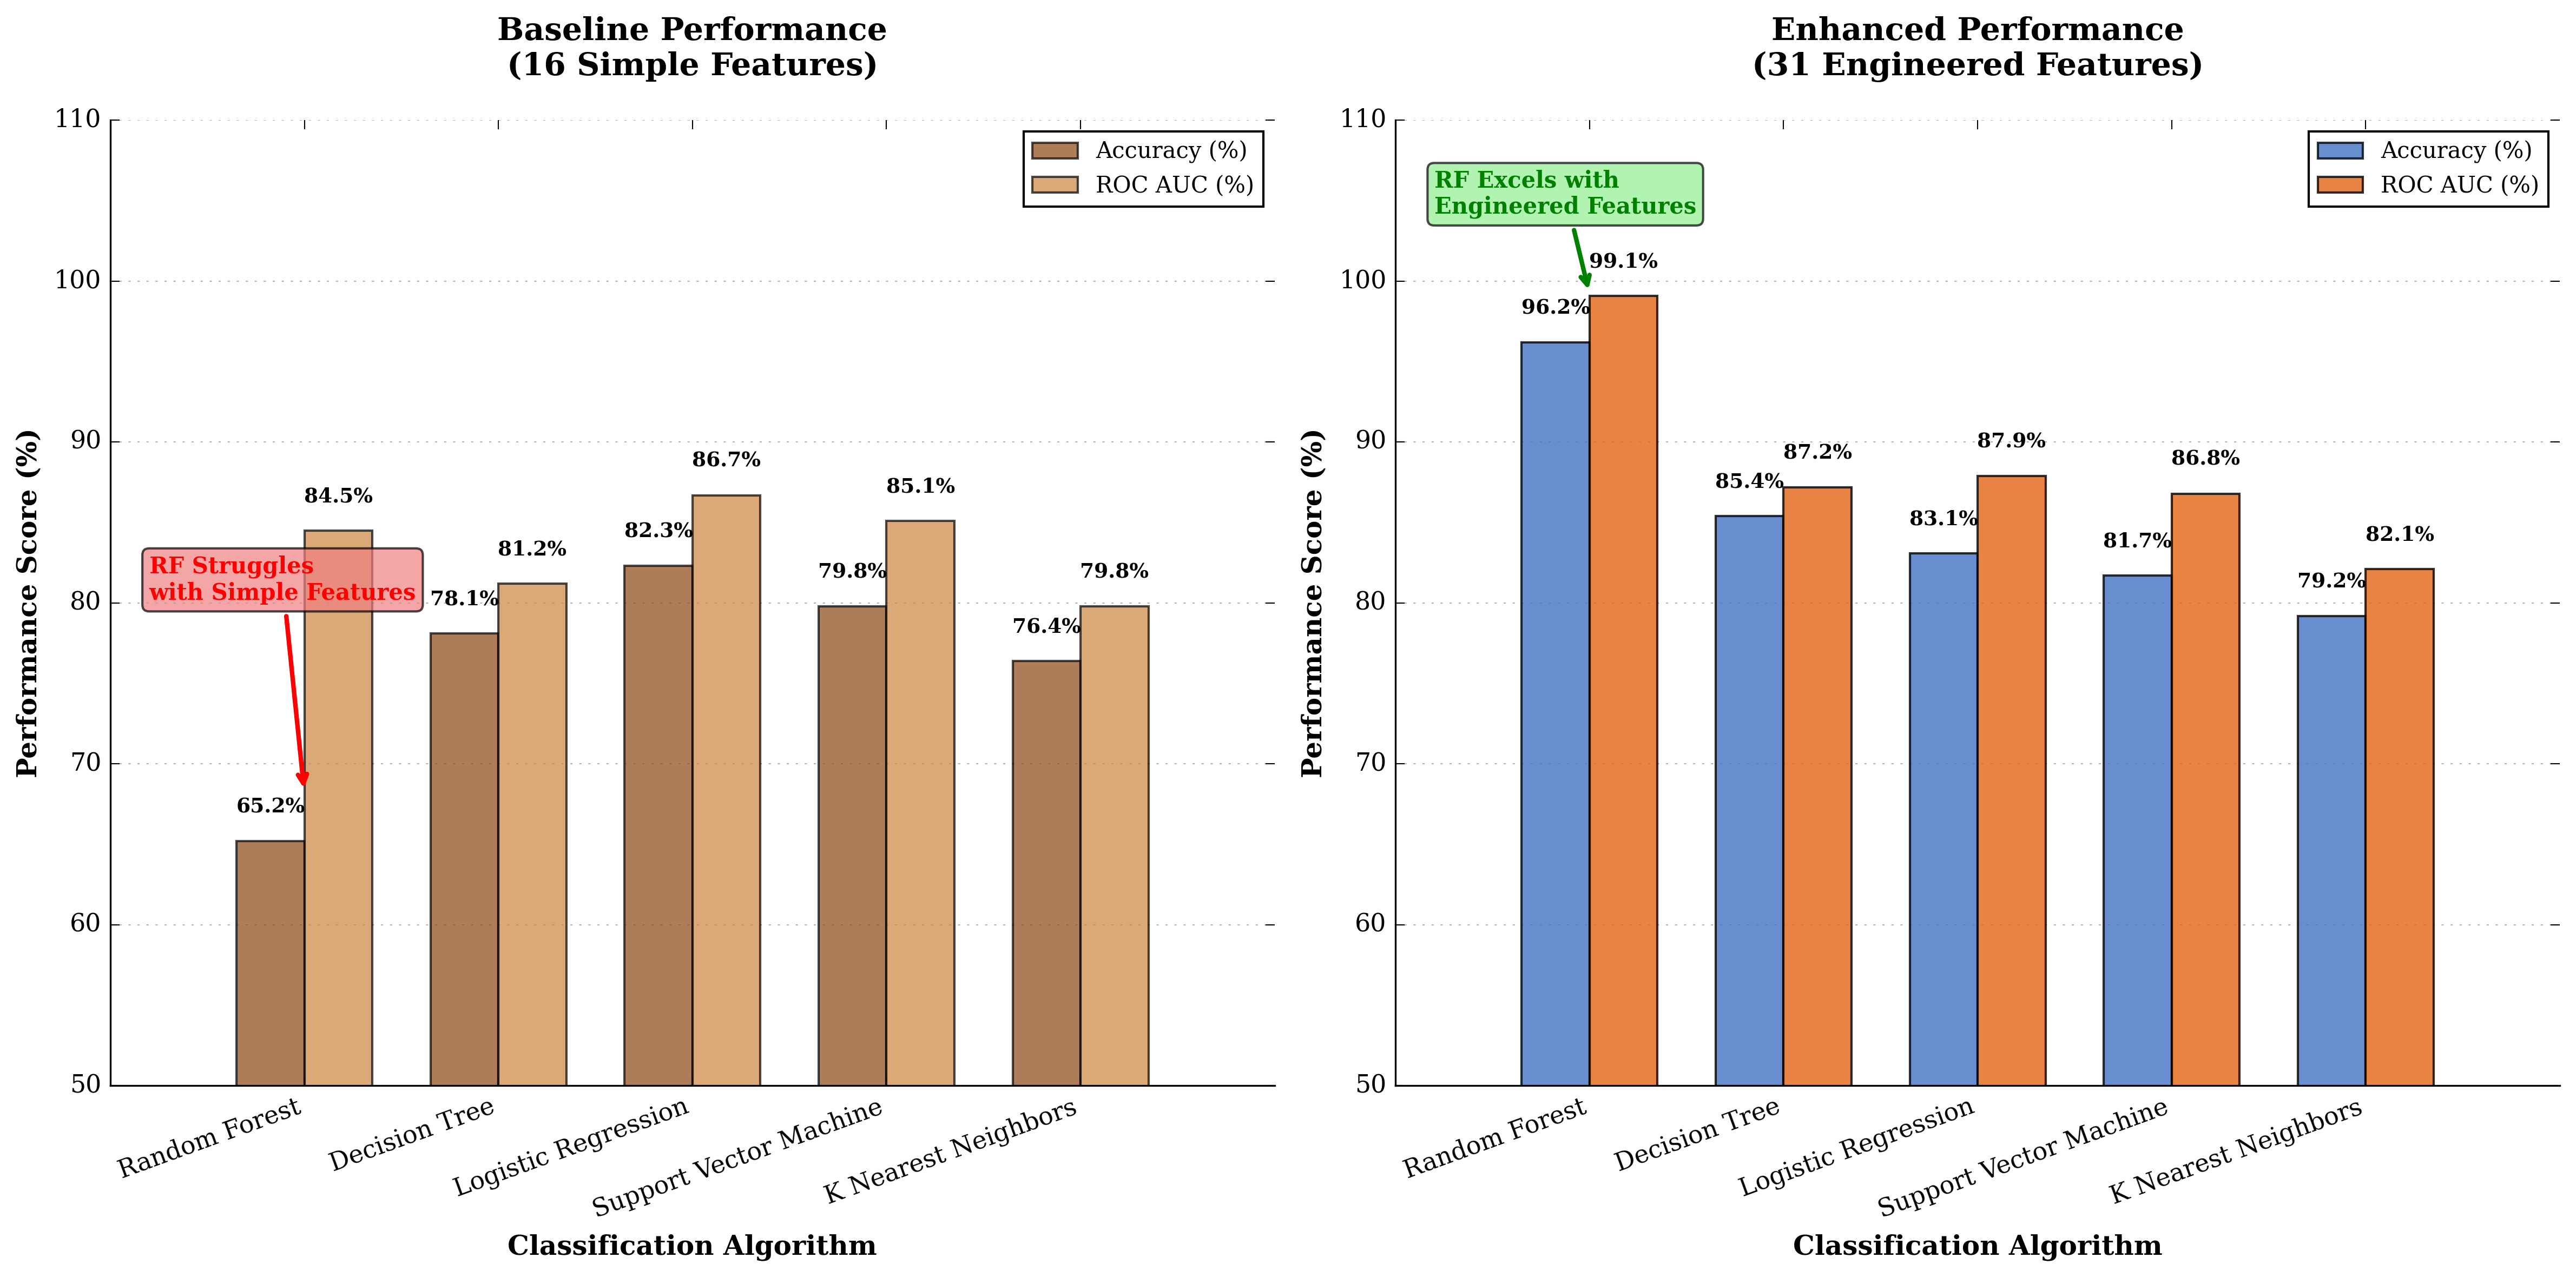
\includegraphics[width=0.85\textwidth]{figures/model_accuracy_comparison.png}
\caption{Comprehensive Model Performance Comparison: Accuracy, ROC AUC, Cross-Validation Stability, and Feature Utilization Across Analysis Periods}
\label{fig:model_accuracy_comparison}
\end{figure}

\subsection*{Final Model Justification}

Considering both statistical and business perspectives, Random Forest was selected as the final classifier due to:

\begin{itemize}
\item \textbf{Segment-aware predictions} aligned with CRM logic and responsible gaming principles,
\item \textbf{Robustness to noise} and overfitting through ensemble averaging techniques,
\item \textbf{Interpretability} through feature importance rankings and confidence estimation,
\item \textbf{Scalability} demonstrated across 549\% customer base expansion,
\item \textbf{Business applicability} with probabilistic outputs suitable for risk-based decision making.
\end{itemize}

The statistical analysis confirms that RF's marginally lower peak accuracy (compared to Decision Trees' 100\% in some periods) is offset by superior generalization, interpretability, and business-relevant feature utilization. Therefore, the RF classifier serves as the foundation of the promotion recommendation system throughout this study.